%This is a LaTeX template for homework assignments
\documentclass{article}
\usepackage[utf8]{inputenc}
\usepackage{amsmath}
\usepackage{amsfonts} 
\usepackage{setspace}
\usepackage{amssymb}
\usepackage{amsmath,bm}
\usepackage{amsthm}
\usepackage{graphicx}
\usepackage{hyperref}
\hypersetup{
    colorlinks=true,
    linkcolor=blue,
    filecolor=magenta,      
    urlcolor=cyan,
    pdftitle={Overleaf Example},
    pdfpagemode=FullScreen,
    }
\urlstyle{same}
\doublespacing
\begin{document}

\section*{Homework 6 Key}
 
\begin{enumerate}%starts the numbering

\item Which of the following functions are well-behaved over the given intervals?
    \begin{enumerate}
    \item $g(x)=\exp(ax),x\in[0,1]$ yes, it is continuous when you take the limit, normalized when you take the integral, and differentiable when you take the derivative.
    \item $g(x)=\frac{1}{x}, x\in[1,2]$ yes, it is continuous when you take the limit, normalized when you take the integral, and differentiable when you take the derivative.
    \item $g(x)=|x|,x\in[-1,1]$ No, it is not discontinuous at x=0, sharp turn.
    \end{enumerate}
\item $\Lambda \approx 16\frac{E}{U_0}(1-\frac{E}{U_0})\exp(-2L\sqrt{\frac{2}{m\hbar^2}(U_0-E)}$\
    \begin{enumerate}
    \item Reducing $E$ and $U_0$ by $10\%$:
    \\ $\Lambda' \approx 16\frac{.9E}{.9U_0}(1-\frac{.9E}{.9U_0})\exp\left(-2L\sqrt{\frac{2}{m\hbar^2}(.9U_0-.9E)}\right)$
    \\ $\Lambda' \approx \exp\left(-2L\sqrt{\frac{2}{m\hbar^2}(U_0-E)}\sqrt{0.9}\right)$
    \item Reducing $L$ by $10\%$:
    \\ $\Lambda \approx 16\frac{E}{U_0}(1-\frac{E}{U_0})\exp(-2*0.9L\sqrt{\frac{2}{m\hbar^2}(U_0-E)}$
    \\ $\sqrt{0.9}<0.9$ so B
    
    \end{enumerate}
\item Make a publication-quality plot of the normalized probability distribution for a particle
in a 1D box of length L in its n = 10 state versus dimensionless position (x = x/L).
Superimpose the classical probability distribution on the same graph. Make sure both axes
have numerical values and proper tick marks.
    \\\centerline{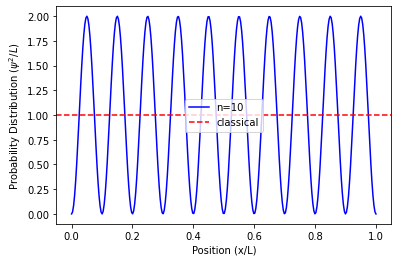
\includegraphics[scale=0.7]{download.png}}
\item Come back next week!
\item 3D harmonic oscillator has potential energy given by: 
    \begin{gather*} V(x,y,z)=\frac{1}{2}k_xx^2+\frac{1}{2}k_yy^2+\frac{1}{2}k_zz^2
    \end{gather*}
    \begin{enumerate}
    \item Find eigenvalues of 3D harmonic oscillator.
    \\ $\hat{H}\psi=E\psi$
    \\ $\hat{H}= \frac{\hbar^2}{2m}\frac{d}{dx}+\frac{1}{2}k_xx^2+\frac{1}{2}k_yy^2+\frac{1}{2}k_zz^2$
    \\ $\hat{H_x}= \frac{\hbar^2}{2m}\frac{d}{dx}+\frac{1}{2}k_xx^2$
    \\ $\hat{H_y}= \frac{\hbar^2}{2m}\frac{d}{dx}+\frac{1}{2}k_yy^2$
    \\ $\hat{H_z}= \frac{\hbar^2}{2m}\frac{d}{dx}+\frac{1}{2}k_zz^2$
    \\ $E=(n+\frac{1}{2})h\nu$ for a 1D harmonic oscillator
    \\ $E=(n_x+\frac{1}{2})h\nu+(n_y+\frac{1}{2})h\nu+(n_z+\frac{1}{2})h\nu$
    \\ $E=(n_x+n_y+n_z+\frac{3}{2})h\nu$ for 3D harmonic oscillator
    \item For an anisotropic 3D harmonic oscillator $k_x=k_y=\frac{1}{3}k_z$. Calculate the degeneracy for lowest 10 levels.
    \\ $V(x,y,z)=\frac{1}{2}k_xx^2+\frac{1}{2}k_yy^2+\frac{1}{2}k_zz^2$
    \\ $E=(n_x+n_y+n_z+\frac{3}{2})h\nu$
    \\ $\omega=\frac{1}{2\pi}\sqrt{\frac{k}{m}}$ and $\hbar=\frac{h}{2\pi}$
    \\ $E=(n_x+n_y+\frac{1}{\sqrt{3}} n_z+\frac{3}{2})\hbar\omega;\forall n\in\mathbb{N}$ so test out numbers
    \\ lowest state $(n_x,n_y,n_z)=0$: (0,0,0) degeneracy = 1
    \\ 2nd lowest $(n_x,n_y,n_z)=1$: (1,0,0);(0,1,0) degeneracy = 2
    \\ 3rd lowest $(n_x,n_y,n_z)=\sqrt{3}$: (0,0,1) degeneracy = 1
    \\ 4th lowest $(n_x,n_y,n_z)=2$: (2,0,0);(0,2,0);(1,1,0) degeneracy = 3
    \\ 5th lowest $(n_x,n_y,n_z)=1+\sqrt{3}$: (1,0,1);(0,1,1) degeneracy = 2
    \\ 6th lowest $(n_x,n_y,n_z)=3$: (3,0,0);(0,3,0);(1,2,0);(2,1,0) degeneracy = 4
    \\ 7th lowest $(n_x,n_y,n_z)=2\sqrt{3}$: (0,0,2) degeneracy = 1
    \\ 8th lowest $(n_x,n_y,n_z)=2+\sqrt{3}$: (1,1,1);(2,0,1);(0,2,1) degeneracy = 3
    \\ 9th lowest $(n_x,n_y,n_z)=4$: (4,0,0);(0,4,0);(3,1,0);(1,3,0);(2,2,0) degeneracy = 5
    \\ 10th lowest $(n_x,n_y,n_z)=1+2\sqrt{3}$: (1,0,2);(0,1,2)degeneracy = 2
    \end{enumerate}
\item  A particle of mass m is in a 2D box. Initially (t = 0), the box has sides S1 and S2 with
lengths L and 4L, respectively. Then, side S2 starts to shrink according to the expression
4L −0.5Lt.
How will the energy gap between the 2nd and 3rd energy levels for this system change as
a function of time? For simplicity, you can focus in the cases where t changes in one unit
from 0 to 7. (Extra credit if you can work out the fully general case).
For a 2D particle in a box of side lengths s1 and s2, the energy is:

\\ $E=\frac{h^2}{8m}(\frac{n_x^2}{a^2}+\frac{n_y^2}{b^2})$
\\ $E_t=\frac{h^2}{8m}\left(\frac{2}{L}+\frac{1}{(4L-0.5Lt)^2}\right)-\frac{h^2}{8m}\left(\frac{1}{L}+\frac{2}{(4L-0.5Lt)^2}\right)$ for energy levels when $L_x>L_y$ this applies when t=0,1,2,3,4,5
\\ Degeneracy at t=6
\\ $E_{t=6}=\frac{h^2}{8m}\left(\frac{2}{L}+\frac{2}{(4L-0.5Lt)^2}\right)-\frac{h^2}{8m}\left(\frac{1}{L}+\frac{2}{(4L-0.5Lt)^2}\right)$ for energy level when $L_x=L_y$
\\ $E_{t=6}=\frac{h^2}{8m}\left(\frac{2}{L}+\frac{1}{(4L-0.5Lt)^2}\right)-\frac{h^2}{8m}\left(\frac{2}{L}+\frac{1}{(4L-0.5Lt)^2}\right)$ for energy level when $L_x=L_y$
\\ At t=7 $L_x<L_y$
\\ $E_{t=7}=\frac{h^2}{8m}\left(\frac{1}{L}+\frac{2}{(4L-0.5Lt)^2}\right)-\frac{h^2}{8m}\left(\frac{2}{L}+\frac{1}{(4L-0.5Lt)^2}\right)$

\end{enumerate}%ends the numbering
\href{https://github.com/lexinsea/teaching/tree/main/quantum-chemistry}{Click here if you are interested in my code.}
\end{document}